%\documentclass{acm_proc_article-sp}

\documentclass{article}

\usepackage{mathpartir}
\usepackage{turnstile}
\usepackage{amssymb}
\usepackage{amsmath}
\usepackage{stmaryrd}
\usepackage{graphicx}
\usepackage{epsfig}
\usepackage{subfigure}
\usepackage{listings}
\usepackage{natbib}
\usepackage{verbatim}
\usepackage[utf8]{inputenc}
\usepackage[T1]{fontenc} 
\usepackage[hyphens]{url}
\lstset{language=ml}
\lstset{commentstyle=\textit}
\lstset{mathescape=true}
\lstset{backgroundcolor=,rulecolor=}
\lstset{frame=single}
\lstset{breaklines=true}
\lstset{basicstyle=\ttfamily}

\DeclareMathOperator{\wf}{wf}
\DeclareMathOperator{\acyclic}{acyclic}
\DeclareMathOperator{\Linear}{Linear}
\DeclareMathOperator{\NonLinear}{NonLinear}
\DeclareMathOperator{\range}{range}
\DeclareMathOperator{\FV}{FV}
\DeclareMathOperator{\LFV}{LFV}
\DeclareMathOperator{\rule-fun}{rule-fun}

\begin{document}

\title{Casanova: \\ a declarative language for safe games}

\author{
Giuseppe Maggiore \and Renzo Orsini \and Michele Bugliesi \\
\{maggiore,orsini,bugliesi\}@dais.unive.it
}

\date{}

\maketitle

\begin{abstract}
Games are extremely complex pieces of software which give life to animated virtual worlds. Games require complex algorithms, large worlds filled with many intelligent entities and high-quality graphics, and it all must run in real time.

Building general, high-performance frameworks capable of representing any virtual world has, until now, proven to be an elusive task; existing solutions either sacrifice performance (X3D browsers) or generality (game engines).

In this paper we present a model that formalizes our notion of a correct game. This model gives all the important properties that game developers struggle to maintain by hand, that is the strong normalization of the \texttt{tick} function, the independence from the order of the ticks of each entity, and the fact that all active entities of the game state must be ticked exactly once. We define the Casanova language around this model, with the aim of achieving the threefold objective of creating games that are correct, declarative (and thus simpler to write) and fast to run.

We will use a linear type system to enforce the uniqueness of our entities (to ensure exactly one tick for each) and to ensure that ticks do not have overlapping effects. We will impose certain restrictions on the state to avoid infinite loops in the update function (in the shape of cyclic references) and we will use a specialized type system to make sure that all the active coroutines of the game will always yield.
\end{abstract}

\begin{comment}
\category{D.1.1}{Programming Techniques}{Applicative (Functional) Programming} 
\category{D.2.2}{Soft\-ware Engineering}{Software Libraries}[Design Tools and Techniques]
\category{D.2.13}{Soft\-ware Engineering}{Reusable Software}[Domain engineering, Reusable libraries, Reuse models]
\category{D.3.3}{Programming Languages}{Language Constructs and Features}
\category{D.3.4}{Pro\-gramming Languages}{Processors}[Optimization, Run-time environments]
\category{H.5.1}{Information Systems}{Information Interfaces and Presentation}[Multimedia Information Systems]

\terms{Games,Performance,Languages}

\keywords{games, compilation}
\end{comment}

\section{Game Model}
\label{sec:game_model}
%%%%%%%%%%%%%%%%%%%%%%%%%%%%%%%%%%%%%%%%%%%%%%%%
% Game Model
%%%%%%%%%%%%%%%%%%%%%%%%%%%%%%%%%%%%%%%%%%%%%%%%

In this section we will define our notion of a correct game. We observe a series of existing game genres, and we break them down into three fundamental building blocks: entities, rules and behaviors.

Entities represent physical and logical objects; ships, asteroids, projectiles, chairs, timers and effect auras are all entities. Entities follow certain rules, which are verified (run) at every tick of the simulation engine. These rules may be physical (no entities may share the same location) or logical (every item has an active aura that influences the surroundings: a chair makes a place more relaxing for characters who then are less prone to attacking). Rules are synchronous with respect to the game tick. Behaviors represent aspects of the game which are asynchronous to the tick function, for example AIs (which perform single actions that span many ticks) and level activators (which wait for certain conditions to be met before offering access to the next gaming stage).

We now present a simple breakdown of games in terms of entities, rules and behaviors; this list is not omnicomprehensive, but it spans various very different game genres (action games, strategy games, role playing games, arcade games):
\begin{itemize}
\item first person shooters:
\begin{itemize}
\item entities are: characters, projectiles, weapons, obstacles, buildings
\item rules are: physics, projectiles damage, picking up weapons, being in cover
\item behaviors are: bot AIs, game logic (capture the flag, other variations), player input
\end{itemize}

\item real time strategy:
\begin{itemize}
\item entities are: units, unit squadrons (if present) buildings
\item rules are: physics, movement (flocking), battle resolution, building queues
\item behaviors are: pathfinding, victory conditions, player input
\end{itemize}

\item Sims:
\begin{itemize}
\item entities are: characters, furniture
\item rules are: furniture auras, social interactions
\item behaviors are: pathfinding, AI, player input
\end{itemize}

\item Puzzle Bobble:
\begin{itemize}
\item entities are: bubbles, bubble queue
\item rules are: bubble movement, bubble blowing, bubble generation
\item behaviors are: level victory, player input
\end{itemize}
\end{itemize}

We describe the game $G$ as the pair $(E,B)$ of all the entities and all the behaviors:

$$ G\ =\ (E,B) $$

Entities are pairs $(e,u)$ of an entity $e$ and its update function $u$.

We define the interpretation $\llbracket u \rrbracket_I$ of an update function as a function from an entity and the game state to its updated version. Since entities update by interacting with each other, the update function cannot take as input the entity $e$ alone. We write:

$$ e' = \llbracket u \rrbracket_I(e,G) $$

to denote the update of an entity $e$.

The interpretation $\llbracket b \rrbracket_I$ of a behavior $b$ is defined as the function that updates the entire state by executing a single step of a behavior. A step of a behavior is executed by sequentially executing all of its instructions from the previous point of suspension until the next. A behavior suspends itself by invoking the \texttt{yield} function.

The interpretation of a set of behaviors $B\ =\ {b_1,...,b_m}$ is the concatenation of all the interpretations of all the behaviors:

$$\llbracket B \rrbracket_I\ =\ \llbracket b_1 \rrbracket_I\ \circ\ ...\ \circ\ \llbracket b_n \rrbracket_I$$

We write:

$$ G' = \llbracket B \rrbracket_I(G) $$

to denote the application of a step of all behaviors to the game.

The tick function is defined as the function that given a game state $G=(E,B)$ produces the updated game state $G'$ where all entities have been updated according to their rules and all behaviors have been run for one step:

$$
\begin{array}{lc}
tick(E,B) = G' \\
\mathtt{where} & \ G' = \llbracket B \rrbracket_I((E',\emptyset)) \\
\mathtt{and} & \ E' = \{(\llbracket u \rrbracket_I(e,G),u)\ |\ (e,u) \in E\}\\
\end{array}
$$

Rules enforce certain properties on each entity; behaviors on the other hand may add, remove or modify any aspect of the game. Behaviors may add or remove new behaviors and entities.

\paragraph{Correctness}

We define four properties of a correct game; these properties are related to the tick:

\begin{enumerate}
\item all rules of each entity are applied exactly once
\item rule application is order-independent
\item tick always terminates
\end{enumerate}

These rules are important because:
\begin{enumerate}
\item if a rule is not applied or is applied more than once we risk inconsistent updates, for example an entity which does not move or moves too fast
\item rule application must be order-independent, because all rules represent aspects of the world which happen during one tick; since the tick is the smallest unit of time in a simulation, anything that happens during one tick must behave as if it happened simultaneously
\item tick must always terminate, since otherwise the simulation would hang indefinitely
\end{enumerate}

We now explore a few common mistakes that are commonly performed when coding games by hand. Let us consider a simple game where the entities are asteroids, cannons and projectiles. We define as entities the asteroids, cannons and projectiles. The user clicks a cannon to make it shoot. Rules are:

\begin{itemize}
\item asteroids fall towards the bottom of the screen
\item projectiles move towards the top of the screen
\item asteroids that are hit by a projectile are destroyed
\item projectiles that hit an asteroid are removed
\item cannons that are hit by an asteroid are destroyed
\item the score is incremented by one whenever an asteroid is hit by a projectile
\item asteroids that exit the screen are removed
\end{itemize}

Behaviors are:

\begin{itemize}
\item when a cannon is clicked it shoots a projectile
\item when the score reaches 1000 the game is won
\item when there are no more cannons the game is lost
\end{itemize}

Let us now consider the mistakes that could be made with respect to the three constraints we have seen above (all rules are executed exactly once, rule application is order-independent and tick is strongly normalizing).

If the first constraint is violated, then an asteroid, projectile or cannon may not be updated correctly or may move or collide more than once; moving more than once during the same tick would multiply an entity velocity by a value greater than one, while colliding more than once would increment the score counter too much.

This constraint could be violated very easily by removing or duplicating the same entity from the entity list.

To see a violation of the second constraint let us consider two possible rules in action; let us assume that rules are executed sequentially and their results are stored in place:

\begin{lstlisting}
module Asteroids =
  (* remove asteroids which are destroyed or which are no more visible *)
  asteroids := [a | a <- asteroids, a.Life > 0, a.InScreen]

  (* increment the score by the number of destroyed asteroids *)
  score := score + [a | a <- asteroids, a.Life <= 0].Count * 10

module Projectiles =
  (* increment the score by the number of projectiles that hit their target *)
  score := score + [p | p <- projectiles, p.HasHit].Count

  (* remove projectiles which hit an asteroid or which are no more visible *)
  projectiles := [p | p <- projectiles, p.HasHit = false, p.InScreen]
\end{lstlisting}

If the destroyed asteroids are removed from the state before the score is updated, then the score will never be modified. Projectiles do not suffer from this problem because the score for projectile hits is registered before the hitting projectiles are removed.

This kind of mistake is easy to make and can easily creep in a game, especially as the number of entity types and processing rules grows. Moreover, by splitting the effects on a field (such as \texttt{score}) in different modules it may becomes quite hard to fully understand how an entity is processed during a single tick.

Violations of the last constraint are very dangerous, in that they do not produce a logical mistake but rather they would make the game hang, which is essentially the same as an application crash but even more invasive to the user who then needs to manually kill the game process (an operation that is made even harder when the game is running in fullscreen and has claimed full ownership of the graphics card).
 

\section{The Casanova language}
\label{sec:casanova}
%%%%%%%%%%%%%%%%%%%%%%%%%%%%%%%%%%%%%%%%
% THE CASANOVA LANGUAGE
%%%%%%%%%%%%%%%%%%%%%%%%%%%%%%%%%%%%%%%%

In this section we present the Casanova language syntax, typing rules and semantics. 

\begin{center}
\line(1,0){240}
\end{center}

\textit{Note on syntactic sugar:}

We will use the following syntactic sugar to increase source code readability:

Rather than write:

\begin{lstlisting}
let! _ = b1
in b2
\end{lstlisting}

we can write:

\begin{lstlisting}
do! b1
in b2
\end{lstlisting}

Rather than write:

\begin{lstlisting}
let x = t1
in let y = t2
in t3
\end{lstlisting}

we can write:

\begin{lstlisting}
let x = t1
let y = t2
t3
\end{lstlisting}

\begin{comment}
We may also directly iterate all the elements of a table \texttt{t} by writing:

\begin{lstlisting}
for x in t do
  action
\end{lstlisting}

rather than explicitly using indices or \texttt{head} and \texttt{tail}.
\end{comment}

\begin{center}
\line(1,0){240}
\end{center}

\subsection{Simple Example}

Before we start, we will give a general idea of how the language works with a small example. We will build a very simple game where asteroids enter the screen from the top, scroll down to the bottom at different velocities and then disappear.

A Casanova program is composed of two portions:
\begin{itemize}
\item the state of the game, a series of types arranged hierarchically (typically at least one for the global state and one for the state of each entity); each portion of the game state may contain exactly one rule (a function that computes the new value of the field)
\item the main behavior, which performs a series of instructions on all the mutable fields of the state (those marked as \texttt{Rule T} or \texttt{Var T}; behavior execution is suspended at the \texttt{yield} statement, and resumed at the next tick
\end{itemize}

The state of our simple program is defined as:

\begin{lstlisting}
type Asteroid =
  {
    Y     : Rule float
          :: \(self,y,dt) -> y + dt * self.VelY
        
    VelY  : float        
    X     : float
  }

type GameState =
  {
    Asteroids           
        : Rule(Table Asteroid)
        :: \asteroids -> [a | a <- asteroids && a.Y > 0]
  	    
    DestroyedAsteroids	
        : Rule<int>
        :: \(state,destroyed_asteroids) -> destroyed_asteroids + count([a | a <- !state.Asteroids && a.Y <= 0])
  }
\end{lstlisting}
  
In a type declaration, the \texttt{:} operator means ``has type'', while the \texttt{::} operator means ``has rule''. Rules can access the game state, the current entity and the time delta between the current and previous ticks.

In the state definition above we can see that the state is comprised by a set of asteroids which are removed when they reach the bottom. Removing these asteroids increments a counter, which is essentially the ``score'' of our game. Each asteroid moves according to its velocity.

The initial state is then provided:
\begin{lstlisting}
let state0 =
  {
    Asteroids               = []
    DestroyedAsteroids      = 0
  }
\end{lstlisting}

After defining the state we must give an initial behavior. As can be easily noticed, our game does not generate any asteroids and so the initial state will never change. Since creating asteroids is an activity that certainly must not be performed at every tick (otherwise we could generate in excess of 60 asteroids per second: clearly too many), we need a function that is capable of performing \textit{different} operations on the state depending on time. Since rules perform the \textit{same} operation at every tick, they are unsuited to this kind of processing. Behaviors are built exactly around this need. The behavior for our game is the following:

\begin{lstlisting}
let main state =
  let random = mk_random()
  let rec wait interval =
    {
      let! t0 = time
      do! yield
      let! t = time
      let dt = t - t0
      if dt > interval then
        return ()
      else
        do! wait (interval - dt)
    }  
  let rec behavior() =
    {
      do! wait (random.Next(1,3))
      do! state.Asteroids.Add
      	  {
      	    X     = random.Next(-1,+1)
      	    Y     = 1
      	    VelY  = random.Next(-0.1,-0.2)
      	  }
      if state.DestroyedAsteroids < 100 then
        do! behavior()
      else
        return ()
    }
  in behavior()
\end{lstlisting}
  
Our behavior declares a random number generator and then starts iterating a function that waits between 1 and 3 seconds and then creates a random asteroid. When the number of destroyed asteroids is greater than 100, the function stops and the game ends (games end when their main behavior terminates).

Notice that behaviors are expressed with two different syntaxes: an ML-style syntax for pure terms (those which read the state and simply perform computations) and an imperative-style syntax for impure terms (those which write the state and interact with time such as wait). The imperative syntax loosely follows the monadic syntax of the F\# language, where a monadic block is declared within \texttt{\{\}} parentheses, monadic operations are preceded by either \texttt{do!} or \texttt{let!} and returning a result is done with the \texttt{return} statement.

\subsection{Syntax}
In the remainder of this section we will adopt the following conventions:
\begin{itemize}
\item capitalized items such as \texttt{Program} and \texttt{StateDef} are grammatical elements
\item quoted items such as \texttt{`type'} and \texttt{`GameState'} are keywords that must appear as indicated
\item items surrounded by \texttt{[ ]} parentheses such as \texttt{[EntityName]} are user-defined strings
\end{itemize}

The program syntax starts with the definition of the state (a series of type definitions with rules) and is followed by the entry point (the initial state and the initial behavior):

\begin{lstlisting}
Program  ::= StateDef
             Main
StateDef ::= EntityDefs
\end{lstlisting}

A type definition is comprised of one of various primitive types such as integers, floating point numbers, two- or three- dimensional vectors, etc. combined into any of the usual composite types known to functional programmers such as tuples, functions, records and sum types. Also, type declarations may contain a rule (which is simply a term, even though with the limitation that only pure functional terms are allowed inside rules). Finally, there are two types for describing behaviors; \texttt{UnsafeBehavior T} which represents an unsafe behavior which may never \texttt{yield}, and \texttt{SafeBehavior T} which represents a safe behavior which never loops indefinitely without \texttt{yield}-ing.

\begin{lstlisting}
TypeDef  ::= TypeDef'
           | TypeDef' :: Rule
          
TypeDef' ::= `()' | `int' | `float' | `Vector2' | ...
           | TypeDef $\times$ TypeDef
           | TypeDef $\rightarrow$ TypeDef
           | `{' Labels `}'
           | TypeDef $+$ TypeDef
           | Modifier TypeDef
           | `UnsafeBehavior' TypeDef
           | `SafeBehavior' TypeDef
           | [EntityName]
           
Labels   ::= Label; Labels
           | Label
           
Label    ::= [Name] `:' TypeDef
                     
Rule     ::= Term
\end{lstlisting}

A \texttt{Modifier} for a type definition allows to make a field mutable (\texttt{Rule} or \texttt{Var}), or to use queries to manipulate that field (\texttt{Table}). Also, another important modifier is \texttt{Ref} which can be seen as a programmer annotation that tells the compiler how a certain field is just a pointer to another portion of the state and as such it must not be processed recursively:

\begin{lstlisting}
Modifier  ::= Rule
            | Var
            | Table
            | Ref
\end{lstlisting}

Entities are definied as a series of type definitions with a name which can be referenced anywhere in the state; the last entity to be defined is the game state itself:

\begin{lstlisting}
EntityDefs  ::= `type' `GameState' = TypeDef
              | EntityDef
                EntityDefs

EntityDef   ::= `type' [EntityName] `=' TypeDef
\end{lstlisting}

The various entity names are simply replaced with their type definition in the remainder of the program, according to the $\llbracket \bullet \rrbracket_{\mathtt{MAIN}}$ translation rule:

\begin{mathpar}
\llbracket \mathtt{type\ EntityName\ =\ TypeDef;\ EntityDefs; Main} \rrbracket_{\mathtt{MAIN}} = 
\llbracket \mathtt{EntityDefs; \ Main} \rrbracket_{\mathtt{MAIN}} \mathtt{[EntityName} \mapsto \mathtt{TypeDef]}

\and 

\llbracket \mathtt{TypeDef;\ Main} \rrbracket_{\mathtt{MAIN}} = \mathtt{TypeDef;\ Main}
\end{mathpar}

The actual type definition of the state may be extracted from the program with the $\sigma(\bullet)$ function, which extracts the type definition and erases all the rules from it; this means that two entities may have the same type with different sets of rules. The function inductively removes all rules from a type declaration:

\begin{mathpar}
\sigma(\mathtt{Entity; EntityDefinitions}) = \sigma(\mathtt{EntityDefinitions})
\and 

\sigma(\mathtt{`type GameState = ' TypeDefinition}) = \sigma(\mathtt{TypeDefinition})
\and 

\sigma(\mathtt{T :: rule}) = \sigma(T)
\and 

\sigma(\mathtt{T}_1 \stackrel{\times}{\stackrel{+}{\mathtt{...}}} \mathtt{T}_2) = 
  \sigma(\mathtt{T}_1) \stackrel{\times}{\stackrel{+}{\mathtt{...}}} \sigma(\mathtt{T}_2)
\and 


\and 

\\ (...) \\
\end{mathpar}

A term can be a simple, ML-style functional term (we do not give all these possible definitions because they are fairly known) or an imperative behavior. Functional terms can read variables with the \texttt{!} operator and can use a Haskell-style table-comprehension syntax:

\begin{lstlisting}
Term        ::= `let' [Var] `=' Term 
                `in' Term
              | `letrec' [Var] `=' Term 
                `in' Term
              | `if' Term `then' 
                   Term 
                `else' 
                   Term
              | Term Term
              | !Term
              | `add' Term Term
              | ... (* other ML-style terms: fun, types, head, tail for tables, etc. *)
              | [ Term | Predicates ]
              | `{' Behavior `}'
              
Predicates  ::= $\epsilon$
              | [Var] `<-' Term, Predicates
              | Term, Predicates
\end{lstlisting}

A behavior defines an imperative coroutine that is capable of reading and writing the state and manipulating time. Behaviors can be freely mixed with terms. The simplest behavior simply returns a result with \texttt{return}. The result of a behavior can be plugged inside another behavior with \texttt{let!}, which behaves like a monadic binding operator. A variable can be modified inside a behavior with \texttt{:=} or \texttt{add}; a behavior can suspend itself until the next tick (\texttt{yield}) and it may read the current time with \texttt{time}.

Behaviors can be combined into more complex behaviors with a small set of combinators. A behavior may spawn another behavior with \texttt{run}, be executed in parallel with another behavior with $\vee$ or $\wedge$, be suspended until another behavior completes ($\Rightarrow$), be repeated indefinitely (\texttt{repeat}) and be forced to execute in a single tick (\texttt{atomic}):

\begin{lstlisting}
Behavior    ::= `return' Term
              | `let!' [Var] `=' Term
                `in' Term
              | Term := Term
              | `yield'
              | `time'
              | `run' Term
              | Term $\vee$ Term
              | Term $\wedge$ Term
              | Term $\Rightarrow$ Term
              | `repeat' Term
              | `atomic' Term
\end{lstlisting}

The main program is comprised of two terms: the initial state and the initial behavior:

\begin{lstlisting}
Main   ::= `let' state0 = Term
           `let' main = Term
\end{lstlisting}


\subsection{Type System}
Our language is strongly typed. We will omit some type declarations when obvious, and our language will make use of type inference. Typing rules for ML-style terms are the usual ML-style typing rules; for example:

\begin{mathpar}
\inferrule
  {\Gamma \vdash t_1:U \\\\ \Gamma,x:U \vdash t_2 : V}
  {\Gamma \vdash \mathtt{let}\ x \mathtt{ = } t_1\ \mathtt{in}\ t_2\ :V}
\quad \textsc {LET}

\and

\inferrule
  {\Gamma \vdash c:bool \\\\ \Gamma \vdash t_1 : T \\\\ \Gamma \vdash t_2 : T}
  {\Gamma \vdash \mathtt{if}\ c\ \mathtt{then}\ t_1\ \mathtt{else}\ t_2 : T}
\quad \textsc {IF}

\and

\inferrule
  {\Gamma \vdash r:Var\ T}
  {\Gamma \vdash !r : T}
\quad \textsc {VAR-GET}

\and

\inferrule
  {\Gamma \vdash r:Rule\ T}
  {\Gamma \vdash !r : T}
\quad \textsc {RULE-GET}

\and

\\ (...)

\end{mathpar}

Table comprehensions are types thusly:

\begin{mathpar}
\inferrule
  {\mathtt{decls(} \Gamma \mathtt{,ts)} \vdash t_1:T}
  {\Gamma \vdash \mathtt{[}\ t_1\ \mathtt{|}\ t_s\ \mathtt{]}\ :Table\ T}
\quad \textsc {TABLE}

\and

\mathtt{decls(} \Gamma \mathtt{,} \epsilon \mathtt{)} = \Gamma

\and

\inferrule
  {\Gamma \vdash t:Table\ T}
  {\mathtt{decls(} \Gamma \mathtt{,(x} \leftarrow \mathtt{t, ts))} = \mathtt{decls((} \Gamma \mathtt{,x:T),ts)}}

\and

\inferrule
  {\Gamma \vdash t:bool}
  {\mathtt{decls(} \Gamma \mathtt{,(t, ts))} = \mathtt{decls(} \Gamma \mathtt{,ts)}}

\and

\\ (...)

\end{mathpar}


\paragraph{Linearity}

Our type system needs to ensure that updating each entity of the state is a safe operation, that is the same entity will be updated \textit{exactly} once. The semantics function that we give further in this Section guarantees that all entities are updated \textit{at least} once, but duplicate entities may be updated twice or more. Updating an entity more than once is dangerous because it may lead to unexpected behaviors, but there is another downside to duplicates: with duplicates, rules are no more order-independent. With duplicates, the same entity may be subject to more than one rule, and thus the same entity may be modified twice in (possibly) irreconcilable ways.

We now show a few examples of how we may produce these situations.

A common error is duplication of a field either inside a behavior or at initialization time; for example, given a record type \texttt{T} with two fields \texttt{Position:Rule U} and \texttt{Velocity:Rule U} we may erroneously write:

\begin{lstlisting}
let r:Rule U = mk_cell ...

let (x:T) = 
  {
    Position = r
    Velocity = r
  }
\end{lstlisting}

Another common error is adding to a table an element from the table itself; for example, given a variable \texttt{t} of type \texttt{Rule Table T} we may write:

\begin{lstlisting}
t.add (t.head)
\end{lstlisting}

The final, common error we show is duplicating data with two symmetric rules:

\begin{lstlisting}
Asteroids$_1$
   : Rule(Table Asteroid) 
   :: fun self -> [a | a <- self.Asteroids$_1$ $\cup$ self.Asteroids$_2$, p$_1$ a]

Asteroids$_2$
   : Rule(Table Asteroid) 
   :: fun self -> [a | a <- self.Asteroids$_1$ $\cup$ self.Asteroids$_2$, p$_2$ a]
\end{lstlisting}

unless $p_1 = \neg p_2$ there will be duplicates between $\mathtt{Asteroids}_1$ and $\mathtt{Asteroids}_2$.

To solve this problem we use two techniques; first, we make \texttt{Rule} a \textit{linear} type. Second, we give rules read-only (\texttt{Ref}) access to the state, so that copying an external portion of the state into another field will require a deep cloning of that portion of the state and not just variable sharing.

We do not discuss all the typing rules required to enforce; instead we show some of the most significant:

\begin{mathpar}
\inferrule
  {\Gamma \vdash t : \mathtt{Ref}\ \{l_1:T_1; ... l_n:T_n\}}
  {\Gamma \vdash t.l_i \ :\ \mathtt{Ref}\ T_i}
\quad \textsc {FOREIGN-LOOKUP}

\and

\inferrule
  {\Linear(U) \\\
   \Gamma \vdash t_1 : U \\\\   
   (\Gamma \setminus \LFV(t_1)),x:U \vdash t_2 : V}
  {\Gamma \vdash \mathtt{let}\ x\ \mathtt{=}\ t_1\ \mathtt{in}\ t_2\ :\ V}
\quad \textsc {LINEAR-LET}

\and

\mathtt{where}

\Linear(T) = (\exists \alpha\ |\ \mathtt{Rule}\ \alpha\ \in \range(T))

\and

\NonLinear(T) = \neg \Linear(T)

\LFV(t) = \{(v:\alpha) | (v:\alpha) \in \FV(t)\ \wedge \Linear(\alpha)\}
\end{mathpar}

\paragraph{Behaviors}

We also state another informal restriction, that is function types may not have rules; so, a type such as $(U :: Rule) \rightarrow V$ is forbidden and generates a compile-time error.

The first typing rules for behaviors are the monadic typing rules which allow to build and consume basic behaviors:

\begin{mathpar}
\inferrule
  {\Gamma \vdash x:T}
  {\Gamma \vdash \mathtt{return}\ x :\ UnsafeBehavior\ T}
\quad \textsc {RETURN}

\and

\inferrule
  {\Gamma \vdash t_1 : b_1 \ U \\\\ \Gamma,x:U \vdash t_2 : b_2\ V}
  {\Gamma \vdash \mathtt{let!}\ x\ \mathtt{=}\ t_1\ \mathtt{in}\ t_2 : b_1 \sqcap b_2 \ V}
\quad \textsc {BIND}

\and

\mathtt{where}

SafeBehavior \sqcap \_ = SafeBehavior
\and
\_ \sqcap SafeBehavior = SafeBehavior
\and
UnsafeBehavior \sqcap UnsafeBehavior = UnsafeBehavior

\end{mathpar}

Behaviors may also be suspended for a tick (to wait for an application of all rules or to synchronize between behaviors, for example), they may read the current time (in fractional seconds) or they may spawn other behaviors:

\begin{mathpar}
\inferrule
  {\\}
  {\mathtt{yield} : SafeBehavior\ ()}
\quad \textsc {YIELD}

\and

\inferrule
  {\\}
  {\mathtt{time} : UnsafeBehavior\ float}
\quad \textsc {TIME}

\and

\inferrule
  {\Gamma \vdash t : SafeBehavior\ ()}
  {\Gamma \vdash \mathtt{run}\ t : UnsafeBehavior\ ()}
\quad \textsc {RUN}
\end{mathpar}

Behaviors are the only places where unrestricted modification of the state may happen; behaviors may indiscriminately write any portion of the state:

\begin{mathpar}
\inferrule
  {\Gamma \vdash t_1 : Var\ (Table\ U) \\\\ \Gamma \vdash t_2 : U}
  {\Gamma \vdash \mathtt{add}\ t_1\ t_2 : UnsafeBehavior\ ()}
\quad \textsc {VAR-TABLE-ADD}

\and

\inferrule
  {\Gamma \vdash t_1 : Rule\ (Table\ U) \\\\ \Gamma \vdash t_2 : U}
  {\Gamma \vdash \mathtt{add}\ t_1\ t_2 : UnsafeBehavior\ ()}
\quad \textsc {RULE-TABLE-ADD}

\and

\inferrule
  {\Gamma \vdash t_1 : Var\ U \\\\ \Gamma \vdash t_2 : U}
  {\Gamma \vdash t_1 \mathtt{:=} t_2 : UnsafeBehavior\ ()}
\quad \textsc {VAR-SET}

\and

\inferrule
  {\Gamma \vdash t_1 : Rule\ U \\\\ \Gamma \vdash t_2 : U}
  {\Gamma \vdash t_1 \mathtt{:=} t_2 : UnsafeBehavior\ ()}
\quad \textsc {RULE-SET}
\end{mathpar}

Conditionals on behaviors propagate the least safe of the two behavior types:

\begin{mathpar}
\inferrule
  {\Gamma \vdash c : bool \\\\ \Gamma \vdash t_1 : b_1\ U \\\\ \Gamma \vdash t_2\ :\ b_2\ U}
  {\Gamma \vdash \mathtt{if}\ c\ \mathtt{then}\ t_1\ \mathtt{else}\ t_2\ :\ b_1 \sqcup b_2 U}
\quad \textsc {IF-BEHAVIOR}

\mathtt{where}

UnsafeBehavior \sqcup \_ = UnsafeBehavior
\and
\_ \sqcup UnsafeBehavior = UnsafeBehavior
\and
SafeBehavior \sqcup SafeBehavior = SafeBehavior
\end{mathpar}

We also support a small behavior calculus. Two behaviors may be executed concurrently (the first one that terminates returns its result while the other behavior is discarded), or they may be executed in parallel (when both terminate their results are returned together). A behavior may also act as a guard ($\Rightarrow$) for another behavior, that is until the first behavior does not terminate with a result the second behavior is kept waiting. Finally, a behavior may be repeated indefinitely or it may be forced to run inside a single tick:

\begin{mathpar}
\inferrule
  {\Gamma \vdash t_1 : b_1\ U \\\\ \Gamma \vdash t_2 : b_2\ V}
  {\Gamma t_1 \vee t_2 : b_1 \sqcup b_2\ (U + V)}
\quad \textsc {CONCURRENT}

\and

\inferrule
  {\Gamma \vdash t_1 : b_1\ U \\\\ \Gamma \vdash t_2 : b_2\ V}
  {\Gamma t_1 \wedge t_2 : b_1 \sqcup b_2\ (U \times V)}
\quad \textsc {PARALLEL}

\and

\inferrule
  {\Gamma \vdash t_1 : SafeBehavior\ (U + ()) \\\\ \Gamma \vdash t_2 : U \rightarrow b\ V}
  {\Gamma t_1 \Rightarrow t_2 : b\ V}
\quad \textsc {GUARD}

\and

\inferrule
  {\Gamma \vdash t : SafeBehavior\ ()}
  {\Gamma \vdash \mathtt{repeat}\ t : SafeBehavior\ ()}
\quad \textsc {REPEAT}

\and

\inferrule
  {\Gamma \vdash t :\ b ()}
  {\Gamma \vdash \mathtt{atomic}\ t : UnsafeBehavior \ ()}
\quad \textsc {ATOMIC}
\end{mathpar}

The typing rules on behaviors force them to be written in such a way as to guarantee statically that no behavior will run indefinitely without yielding. This is seen easily because the only two operators capable of looping are \texttt{repeat} and $\Rightarrow$, and both require a \texttt{Safebehavior} as input. 

We now show a small list of dangerous behaviors that are forbidden by our type system:

\begin{lstlisting}
repeat { r := v }

repeat {if cond then r := v else yield}

{ return None } => fun () -> yield
\end{lstlisting}

The inability to eliminate a behavior unless inside another behavior is important because it allows us to force rules to not contain behaviors; thanks to this limitation we can ensure that the execution of rules may only read from the state and never write to it, and so rules can be made to behave as if they are executed simultaneously without risking complex interdependencies. This simplifies many instances of game programming; for example, consider the rules seen in the example at the beginning of the section:

\begin{lstlisting}
Asteroids           
    : Rule(Table Asteroid)
    :: \asteroids -> [a | a <- asteroids && a.Y > 0]
  	    
DestroyedAsteroids	
    : Rule<int>
    :: \(state,destroyed_asteroids) -> destroyed_asteroids + count([a | a <- !state.Asteroids && a.Y <= 0])
\end{lstlisting}

If rules are executed sequentially from top to bottom, then when an asteroid is eliminated that same asteroid will not be available anymore when computing the number of asteroids waiting for deletion.


\subsection{Accepted Programs}

To determine if a game is correct or not we require for it to pass a static analyisis which is comprised of two steps: its state definition must be well-formed (the $\wf(\bullet)$ function) and its \texttt{main} must be typed correctly.

The $\wf(\bullet)$ function requires that a state definition's rules are typed correctly:

\begin{mathpar}
\wf(\mathtt{type [EntityName] = TypeDef;\ EntityDefinitions}) = \wf(\mathtt{TypeDef}, \mathtt{EntityName}) \wedge \wf(\mathtt{EntityDefinitions})
\and

\wf(\mathtt{Primitive}, \mathtt{EntityName}) = \mathtt{true}
\and

\wf(\mathtt{CompositeType(Types)}, \mathtt{EntityName}) = \bigwedge_{\mathtt{T} \in \mathtt{Types}}(\wf(\mathtt{T}, \mathtt{EntityName}))
\and

\wf(\mathtt{Rule\ T\ ::\ rule}) = \wf(\mathtt{T}, \mathtt{EntityName}) \wedge 

\inferrule
  {}
  {\vdash \mathtt{rule}\ : rule-fun(T,EntityName) }

\and

\wf(\mathtt{Var\ T}, \mathtt{EntityName}) = \wf(\mathtt{T}, \mathtt{EntityName})
\and

\wf(\mathtt{Table\ T}, \mathtt{EntityName}) = \wf(\mathtt{T}, \mathtt{EntityName})
\and

\wf(\mathtt{Foreign\ T}, \mathtt{EntityName}) = \mathtt{true}

\and

\\\\
\mathtt{where}

\rule-fun(T,\mathtt{EntityName}) = \mathtt{Foreign(GameState)} \times \mathtt{Foreign(EntityName)} \times \mathtt{T} \times \mathtt{float} \rightarrow \mathtt{T}
\end{mathpar}

Given a game source:
\begin{lstlisting}
StateDefinition

let state0 = $t_1$
let main   = $t_2$
\end{lstlisting}

its compilation succeeds if the following is satisfacted:

\begin{mathpar}
\wf(\mathtt{StateDefinition}) \wedge \\
   \vdash t_1 : \sigma(\mathtt{StateDefinition}) \wedge \\
   \vdash t_2 : \sigma(\mathtt{StateDefinition}) \rightarrow \mathtt{SafeBehavior()}
\end{mathpar}


\subsection{Semantics}

We now define the semantics function of a Casanova program.

We start by defining our memory model. Our memory is defined as a map from rules and variables into values:

\begin{lstlisting}
m = $\epsilon$
  | m[r $\rightarrow$ v]
  | m[r $\Rightarrow$ v]
\end{lstlisting}

\texttt{m[r $\rightarrow$ v]} means that \texttt{r}, which has type \texttt{Var T} or \texttt{Rule T} has value \texttt{v}, while \texttt{m[r $\Rightarrow$ v]} means that \texttt{r}, which has type \texttt{Rule T}, has a pending assignment of value \texttt{v}. The execution of rules does not modify assignments of the form \texttt{m[r $\rightarrow$ v]}, and it will only add assignments of the form \texttt{m[r $\Rightarrow$ v]}. After all rules have been executed, then we use the compacting function $\oplus$:

\begin{lstlisting}
$\oplus$($\epsilon$) = $\epsilon$
$\oplus$(m[r $\rightarrow$ v]) = ($\oplus$m)[r $\rightarrow$ v]
$\oplus$(m[r $\Rightarrow$ v]) = ($\oplus$m)[r $\rightarrow$ v]
\end{lstlisting}

The \texttt{!} operator (valid on both rules and variables) is defined as:

\begin{lstlisting}
!r (m[r' $\rightarrow$ v]) = if r = r' then v else !r m
!r (m[r' $\Rightarrow$ v]) = !r m
\end{lstlisting}

variables may never be null, since there is no way of declaring a variable without initializing it at the same time; this way we are assured that variable lookups will always succeed in finding a value.

The \texttt{:=} operator (valid on both rules and variables) is defined as:

\begin{lstlisting}
(r := v) m = m[r $\rightarrow$ v]
\end{lstlisting}

Notice that \texttt{:=} cannot be used inside the body of a rule, thanks to the limitation that the type system imposes that unrestricted assignments can only happen inside behaviors.

We can now define the \texttt{update\_rules} function, which builds the program that will run all the rules; this program takes as input the memory and after each imperative statement it returns the modified memory. The \texttt{update\_rules} function inductively processes the state and applies each rule it finds. The function does not recursively process those portions of the state with type \texttt{Foreign T} for some \texttt{T}.

The \texttt{update\_rules} function traverses all entity definitions starting from the beginning of the program; it also invokes the compacting function $\oplus$ to apply all the pending changes caused by all the rule executions:

\begin{lstlisting}
update_rules (StateDefinition; Main) m =
  $\oplus$(update_state StateDefinition m)

update_state (type EntityName = TypeDef; EntityDefinitions) =
  entities_update[(update_state EntityName EntityName) $\mapsto$ entity_update]
  where
    entities_update = update_state EntityDefinitions
  and
    entity_update = update_entity TypeDef TypeDef
    
update_state (type GameState = TypeDef) =
  update_entity TypeDef TypeDef
\end{lstlisting}

The \texttt{update\_state} function inductively processes type definitions; on each type definition it goes in search for rules and applies those rules with the \texttt{update\_entity} function:

\begin{lstlisting}
update_entity E T m (s,(e:E),(t:T),dt) = m (* when T is a primitive type such as (), int, ... *)

update_entity E (U $\rightarrow$ V) m (s,e,f,dt) = m

update_entity E (SafeBehavior T) m (s,e,f,dt) = m

update_entity E (UnsafeBehavior T) m (s,e,f,dt) = m

update_entity E (Foreign T) m (s,e,f,dt) = m

update_entity E (U $\times$ V) m (s,e,(u,v),dt) = 
  update_entity E U (update_entity E V m (s,e,v,dt)) (s,e,u,dt)

update_entity E (U $+$ V) m (s,e,(Left u),dt) = update_entity E U m (s,e,u,dt)

update_entity E (U $+$ V) m (s,e,(Right v),dt) = update_entity E V m (s,e,v,dt)

update_entity E ({l1:T1,...,ln:Tn}) m (s,e,r,dt) = 
  update_entity E T1 (... (update_entity E T1 m (s,e,r.ln,dt)) ... ) (s,e,r.l1,dt)

update_entity E ([EntityName]) m (s,e,e',dt) = (update_entity [EntityName] [EntityName]) m (s,e',e',dt)

update_entity E (Var T) m (s,e,r,dt) = update_entity E T m (s,e,!r m,dt)

update_entity E (Table T) m (s,e,t,dt) = [update_entity E T m (s,e,x,dt) | x $\leftarrow$ t]

update_entity E (Rule T :: rule) m (s,e,r,dt) = 
  update_entity E T (m[r $\Rightarrow$ ($\llbracket \mathtt{rule} \rrbracket_I$ m (s,e,!r m,dt)]) (s,e,!r m,dt)
\end{lstlisting}

Where $\llbracket \bullet \rrbracket_I\ \mathtt{m}$ is the well-known semantics of the pure lambda calculus, augmented with the rule that:

$\llbracket !r \rrbracket_I\ \mathtt{m}$ \texttt{ = !r m}.

Behavior semantics is simpler than rule semantics. We update a list of behaviors, where each behavior may modify the memory or run new behaviors. Each behavior may also perform regular functional computations which are processed according to $\llbracket \bullet \rrbracket_I \mathtt{m}$.

We define the \texttt{update\_behaviors} function which folds the \texttt{update\_behavior} over all behaviors; each single behavior update modifies the memory and returns a set of behaviors to run at the next update:

\begin{lstlisting}
update_behaviors ({b1,...,bn},m) =
  ((b1',bs'),m'')
  where 
    (),b1',m' = update_behavior m b1
  and
    bs',m'' = update_behaviors ({b2,...,bn},m')
\end{lstlisting}

The \texttt{update\_behavior} function executes a behavior until the next \texttt{yield}, immediately writing assignments to the memory; we omit the definition of this function for regular pure functional terms, and instead give it only for behavior terms:

\begin{lstlisting}
update_behavior m (return v) = v,{},m

update_behavior m (let! _ = yield in t) = (),(t),m

update_behavior m (let! _ = (run b) in t) = 
  v,(b,b'),m'
  where
    v,b',m' = update_behavior m (t)

update_behavior m (let! _ = (r := v) in t) = 
  v,b,m'
  where
    v,b,m' = update_behavior (m[r $\rightarrow$ v]) (t)

update_behavior m (let! x = !r in t) = 
  v,b,m'
  where
    v,b,m' = update_behavior (($\lambda$x . t) (!r m)) m

update_behavior m (let! x = !r in t) = 
  v,b,m'
  where
    v,b,m' = update_behavior (($\lambda$x . t) (!r m)) m

update_behavior m (let! x = t1 in t2) = 
  update_behavior (($\lambda$x . t2) t1) m
\end{lstlisting}

The two update functions, one for rules and one for behaviors are combined into the final update function which takes as input the game state, the set of current behaviors and the current memory and which returns the updated behaviors and memory. The state never changes, but the memory it points to may:

\begin{lstlisting}
update Program state bs m =
  bs',m''
  where
    bs',m' = update_behaviors (bs,m)
  and
    m'' = update_rules Program m' state
\end{lstlisting}


\subsection{Correctness}
We have stated in Sec. \ref{sec:game_model} that a correct game according to our model respects the following rules:
\begin{enumerate}
\item all rules of each entity are applied exactly once
\item rule application is order-independent
\item tick always terminates
\end{enumerate}

We will now briefly discuss why our system forces games to respect these rules:
\begin{enumerate}
\item is respected because the semantics function explores the entire state recursively and applies its rules making sure that each rule is applied at least once; the linearity of the \texttt{Rule} type makes sure that the same cell is never processed more than once with one or more rules
\item is respected because rule application cannot access the result of already completed rules because those results are stored in memory as $m[r \Rightarrow v]$ but each rule may only read memory cells of the form $m[r \rightarrow v]$; also, the linearity of the \texttt{Rule} type ensures that no two rules write the same cell with $m[r \Rightarrow v]$, because all $r$'s are distinct
\item is respected because the state is not cyclic (apart from \texttt{Foreign} declarations, which are not processed recursively) and because only behaviors with type \texttt{YieldBehavior} can be run, that is accepted behaviors never run indefinitely without yielding
\end{enumerate}



\section{Compilation}
\label{sec:compilation}
%%%%%%%%%%%%%%%%%%%%%%%%%%%%%%%%%%%%%%%%%%%%%%%%
% Compilation
%%%%%%%%%%%%%%%%%%%%%%%%%%%%%%%%%%%%%%%%%%%%%%%%

In this section we will show an outline of the Casanova compiler. In Fig. \ref{fig:compilation_process} we can see that compilation is a four step process.

In the first step we parse the program source code. The output is an AST which represents the program, with the rules and types as annotations.

The AST is fed to the type checker, which makes sure that the program does not contain incorrect operations. It makes sure that no duplication of \texttt{Rule T} values happens, which would cause inconsistencies when applying rules. The type checker also makes sure that behaviors are typed correctly, thereby ensuring that all behaviors are typed as \texttt{Safebehavior} and thus they do not cycle indefinitely without invoking \texttt{yield}.

The resulting AST is then processed by the F\# translator, which generates F\# code that defines the state and entity types and which implements the semantic function.

The F\# translator also performs some optimizations which we will discuss in the next paragraph.

Finally, the resulting F\# program is compiled by the standard F\# compiler thereby generating a library which can then be used as the game engine for an XNA (Windows PCs, Xbox 360 or Windows Phone 7) or MonoTouch (iPad, iPhone or Android) game.

\begin{figure}
\begin{center}
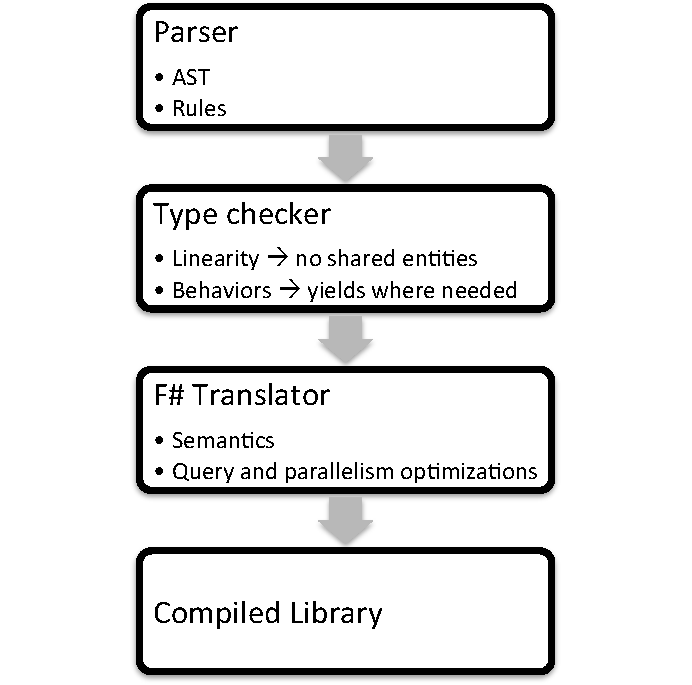
\includegraphics[scale=0.75]{compilation_process.pdf}
\end{center}
\caption{Compilation process}
\label{fig:compilation_process}
\end{figure}


\paragraph{Optimization}

Casanova performs three main optimizations.

The first optimization is a very simple one: memory recycling; even if simple, it can prove very effective in all those platforms (such as the Xbox 360) with a slow garbage collector. Memory recycling means that \texttt{Rule T} fields allocate a double buffer for storing both the $\mathtt{m}[r \rightarrow v]$ value and the $\mathtt{m}[r \Rightarrow v]$ value. Applying the $\oplus \mathtt{m}$ operator simply requires swapping the two buffers. The \texttt{Rule T} datatype is defined as:

\begin{lstlisting}
type Rule<'a> =
  {
    Values              : 'a[]
    FrameIndex          : int ref
  }
  member private this.ValueIndex
    with get() = this.FrameIndex.Value % this.NumValues
  member private this.ValueIndex' 
    with get() = (this.FrameIndex.Value + 1) % this.NumValues
  member this.Value
    with get() = this.Values.[this.ValueIndex]
    and set v' = this.Values.[this.ValueIndex] <- v'
  member this.Value'
    with get() = this.Values.[this.ValueIndex']
    and set v' = this.Values.[this.ValueIndex'] <- v'
\end{lstlisting}

all \texttt{Rule T}'s share the same reference to the current frame index. Whenever we wish to swap the references (that is when we apply the $\oplus$ function) then we just increment the \texttt{FrameIndex} without any need for traversing the entire state to manually set all \texttt{Rule T}'s.

This optimization can be extended to tables: at the beginning of each update, all values of type \texttt{Rule (Table T)} get their \texttt{Value'} cleared; clearing a table does not deallocate its elements: rather, it simply sets the counter of elements to zero, while keeping the previous memory allocated.

This strategy helps reducing the amount of garbage collection needed, sometimes giving large speedups as we can see in Section \ref{sec:benchmarks}.


The second optimization takes advantage of the static constraint that rules are linear: this means that no rules write the same memory location. We also know that rules may not freely write any references. These two facts guarantee thread safety, that is we may run or rules in parallel. Casanova dynamically allocates twice as many threads as the number of cores of the machine. Threads are only used to process lists of entities in the \texttt{GameState}, but no further multi-threading is performed: if an entity should contain many sub-entities those will all be processed sequentially in the same thread. This is needed to avoid creating too many threads; an excessive number of threads may even cause so much overhead that the benefits of parallelization are inferior to the losses in performance caused by the cost of threads.

The $i^{th}$ thread of $n$ will process the $i^{th}$ portion of each top-level table of the game state. This means that if the state is defined as:

\begin{lstlisting}
type GameState = 
  {
    Asteroids   : Table Asteroid
    Projectiles : Table Projectile
  }
\end{lstlisting}

then the $i^{th}$ thread will run the function:

\begin{lstlisting}
let thread state n i =
  for j = i * state.Asteroids.Count / n 
      to (i+1) * state.Asteroids.Count / n do
    update state.Asteroids.[j]
  for j = i * state.Projectiles.Count / n 
      to (i+1) * state.Projectiles.Count / n do
    update state.Projectiles.[j]
\end{lstlisting}

Unless the number of entities is very small or behaviors are very complex and computationally intensive, then the gains obtained by parallelization can be very high; the best results may even divide the duration of a tick by the number of threads, even if this is rarely the case.


The final optimization is query optimization. Nested list comprehensions (also known as ``joins'' in the field of databases) can have high computational costs; for example, the query:

\begin{lstlisting}
type Asteroid =
  {
    CollidingProjectiles 
      : Rule(Table(Foreign(Projectile)))
      :: \(state,self) -> [p | p <- state.Projectiles, collides(self,p)]     
  }
\end{lstlisting}

has a computational complexity of $O(n_p \times n_a) = O(n^2)$, where $n_p$ is the number of projectiles, $n_a$ is the number of asteroids and $n$ is the maximum between the two. Such a complexity is unacceptable when we start having a large number of asteroids and projectiles, because it may severely limit the maximum number of entities supported by the game.

We use the same physical optimization techniques used in modern databases: we build an index to speed up our collision detection. In particular, we observe that most asteroids and projectiles are so far away that testing them for collision does not make sense. We partition the space of the playing area into various blocks and we assign all our projectiles to the blocks they belong to; this operation costs $O(n_p)$ if blocks are a uniform grid and $O(n_p \log n_p)$ if blocks are of variable size and represented with a tree. For each asteroid, we find the blocks it belongs to ($O(n_a)$ or $O(n_a \log n_a)$) and then check for collisions only with the projectiles in those blocks. The final cost of the operation is $O(n)$ for hash maps and $O(n \log n)$ for trees.

An example hash map optimization could be the following. We add the following declaration to the game state:

\begin{lstlisting}
type GameState = 
  {
    ...
    Blocks   : Block[][]
  }
\end{lstlisting}

where a \texttt{Block} contains a list of projectiles.

In the update function we start by clearing the \texttt{Blocks} index and we fill it again with the updated projectiles:

\begin{lstlisting}
let update_state (state:GameState) (dt:float32) =
  for b in state.Blocks do
    b.Clear()
  
  for p in state.Projectiles do
    for b in p.Blocks do
      b.Add p
\end{lstlisting}

Benchmarks show that the costs of rebuilding the index are similar to modifying it, especially for trees. In this sense we confirm a similar result found in.

Collision detection will now become:

\begin{lstlisting}
let update_asteroid (state:GameState) 
                    (self:Asteroid) 
                    (dt:float32) =
  for b in self.Blocks do
    for p in b.Projectiles do
      if collides self p then
        self.CollidingProjectiles.Add p
\end{lstlisting}

A small bottleneck of this computation is the clearing phase, because it forces us to iterate all the blocks (which may be a large number for increased optimization) even if most of those are empty. For this reason, we further augment the state to track those blocks that contain projectiles (and thus which need clearing):

\begin{lstlisting}
type GameState = 
  {
    ...
    NonEmptyBlocks  : Table (BlockIndex)
  }
\end{lstlisting}

Now the update function becomes:

\begin{lstlisting}
let update_state (state:GameState) (dt:float32) =
  for bi in state.NonEmptyBlocks do
    state.Blocks.[bi].Clear()
  
  for p in state.Projectiles do
    for b in p.Blocks do
      b.Add p
      state.NonEmptyBlocks.Add b.Index
\end{lstlisting}

We must stress the importance of this last optimization. By having a function of quadratic complexity in the number of entities we are forcing our game to run with a maximum number of entities. Less entities often make for a less compelling game, because the world is less complex and the challenges are smaller. This class of optimizations allows the game performance to be less dependent on the number of entities. This means that we may design grander worlds with thousands of units and \textit{with no additional development complexity}.

\section{Case Studies}
\label{sec:case_study}
%%%%%%%%%%%%%%%%%%%%%%%%%%%%%%%%%%%%%%%%%%%%%%%%%%%%%%%%%%
% case_study.tex
%%%%%%%%%%%%%%%%%%%%%%%%%%%%%%%%%%%%%%%%%%%%%%%%%%%%%%%%%%

We will now present a more detailed example to see our compiler in action by showing how it handles all the features of an X3D scene: entities and routes. We will consider an X3D scene that contains a looping timer which updates a color that in turn updates the material used when drawing a box:

\begin{lstlisting}[language=xml]
<Scene>
  <ColorInterpolator DEF='myColor'
    keyValue='1 0 0, 0 1 0, 0 0 1, 1 0 0'
    key='0.0 0.333 0.666 1.0'/>
  <TimeSensor DEF='myClock' cycleInterval='10.0' loop='true'/>
  <Shape>
    <Box/>
    <Appearance>
      <Material DEF='myMaterial'/>
    </Appearance>
  </Shape>
  <ROUTE fromNode='myClock' fromField='fraction_changed'
         toNode='myColor' toField='set_fraction'/>
  <ROUTE fromNode='myColor' fromField='value_changed'
         toNode='myMaterial' toField='diffuseColor'/>
</Scene>
\end{lstlisting}

Our compiler produces the following state definition from the above scene:

\begin{lstlisting}
type Scene =
  {
    myColor       : ColorInterpolator
    myClock       : TimeSensor
    myMaterial    : Material
    dynamic_nodes : List<Node>
    script        : Script
  }
\end{lstlisting}

where pointers to all statically known nodes are maintained.

The initialization function for our state initializes a set of local variables, one for each named node, and then builds the actual scene state. Notice that at this point routes are ignored, since they will be used only for the update function:

\begin{lstlisting}
let scene = 
  let myColor = 
       ColorInterpolator(
         keyValue = [ ... ],
         key = [ ... ])
  let myClock = 
       TimeSensor(
         cycleInterval = 10.0,
         loop = true)
  let myMaterial = Material()
  let dynamic_nodes = 
        [
          Shape(
            Value = 
              Box(Appearance(Value = myMaterial)))
        ]
  {
    myColor        = myColor
    myClock        = myClock
    myMaterial     = myMaterial
    dynamic_nodes  = dynamic_nodes
    script         = null
  }         
\end{lstlisting}

After initializing the scene without a script, we can load the script from an external parameter that will be assigned in the linking phase. Loading a script requires passing to it the scene, so that the script may access the scene to manipulate it:

\begin{lstlisting}
scene.script := load_script scene
\end{lstlisting}

The update function invokes the internal update function of all nodes, starting from the statically known and ending with the dynamic ones. Routes are executed in the update function:

\begin{lstlisting}
let update dt = 
  scene.myClock.update dt
  scene.myColor.update dt
  scene.myMaterial.update dt
  for node in scene.dynamic_nodes do
    node.update dt
  scene.script.update dt
  
  myColor.fraction <- myClock.fraction
  myMaterial.diffuseColor <- myColor.value
\end{lstlisting}

It is important to notice that routes in the update function are represented by the actual chains of field updates that need to be performed; there is no overhead when dynamically propagating the update events. Also, if a field does not start a route then there are no ``hidden'' costs as we would have when firing a \texttt{FieldModified} event with no routes listening.


\section{Benchmarks}
\label{sec:benchmarks}
%%%%%%%%%%%%%%%%%%%%%%%%%%%%%%%%%%%%%%%%%%%%%
% BENCHMARKS
%%%%%%%%%%%%%%%%%%%%%%%%%%%%%%%%%%%%%%%%%%%%%

- Windows, Xbox, Wp7 (, iPad?)
- memory recycling
- parallel execution
- query optimization


\bibliographystyle{plain}
\bibliography{references} 

\cite{*}
%\nocite{}

\end{document}
